%!TEX root=report.tex
\subsection{Splines}
Using 9 knots with a year in between and letting the sine and cosine function enter at each knot, one can allow for different seasons. The columns in $X$ can be visualized as in Figure \ref{fig:splines-x-columns}.
\begin{figure}[H]
	\centering
	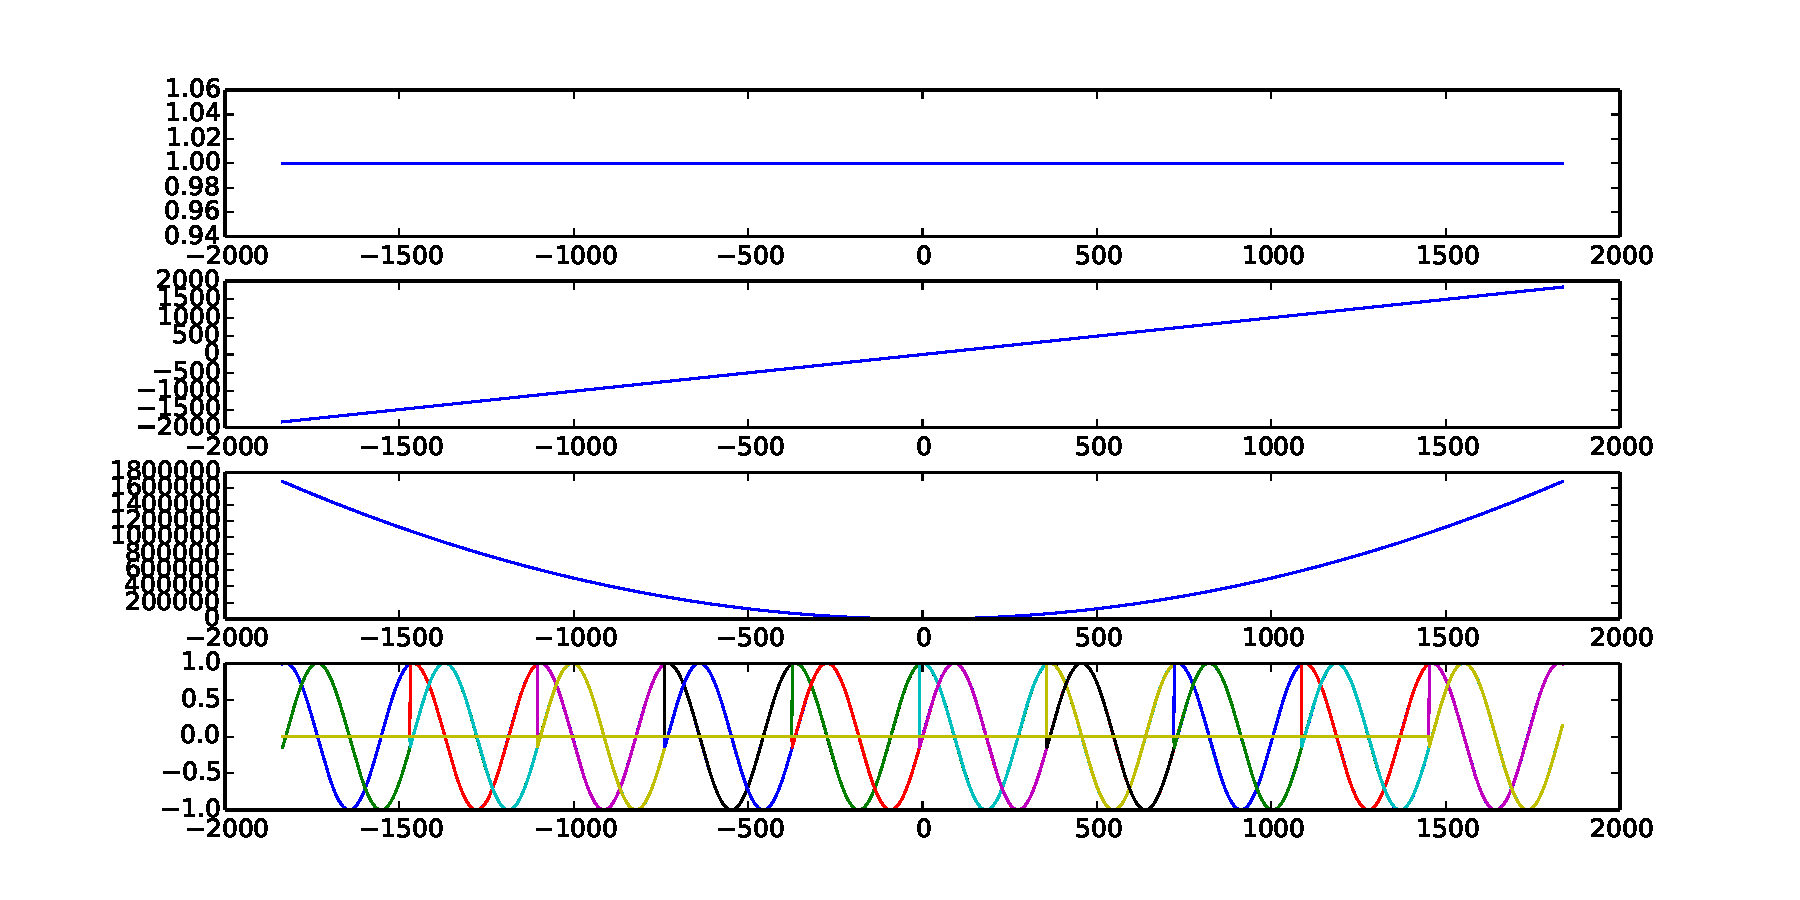
\includegraphics[width=\textwidth]{figures/splines-x-columns}
	\caption{Constant, trend and acceleration in the 3 uppermost plots. Sine and cosine hinge functions in the bottom plot.}
	\label{fig:splines-x-columns}
\end{figure}

A RMSE diagnostic shows that the residuals are indeed smaller (max standard OLS was 0.135).

\begin{figure}[H]
	\centering
	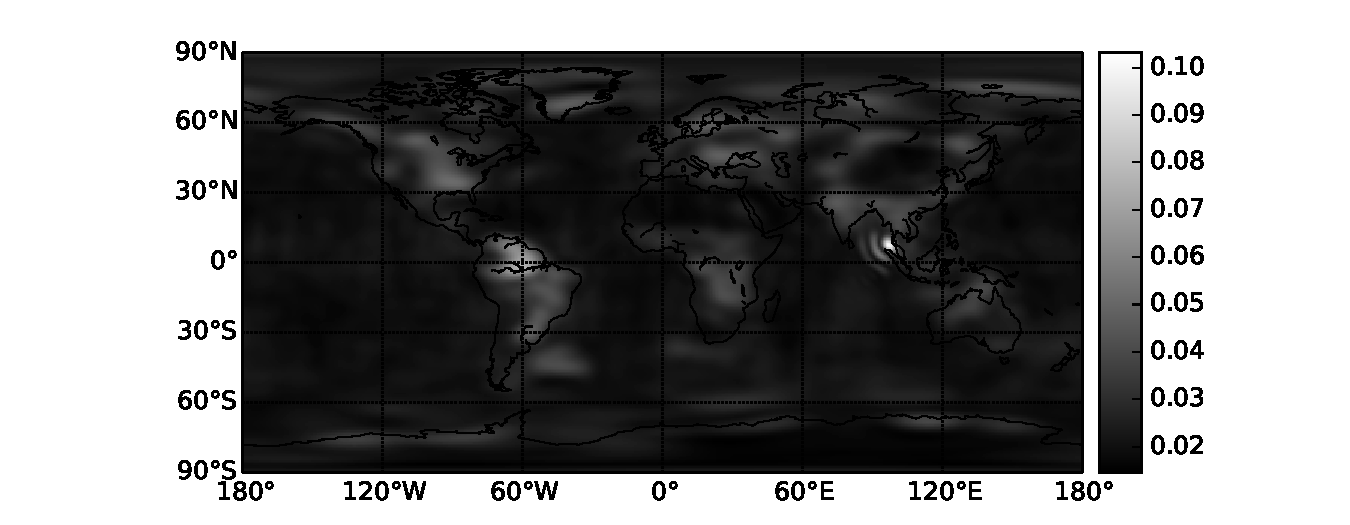
\includegraphics[width=\textwidth]{figures/splines-rmse}
	\caption{RMSE for each position using basis expansion.}
	\label{fig:splines-rmse}
\end{figure}

Looking at the west coast of Greenland now using a basis expansion, the overall fit (Figure \ref{fig:splines-selected-0-fit}) looks improved. For some reason 2009 still causes some issues, which is partially seen in the residuals (Figure \label{fig:splines-selected-0-residual}). Another thing to notices is that the curves are a lot more smooth, but this is simply because only the first 3 frequencies (year, half year and quarter year) was used. This was to prevent the degrees of freedom to drop dramatically, dude to the otherwise huge amount of parameters.
\begin{figure}[H]
	\centering
	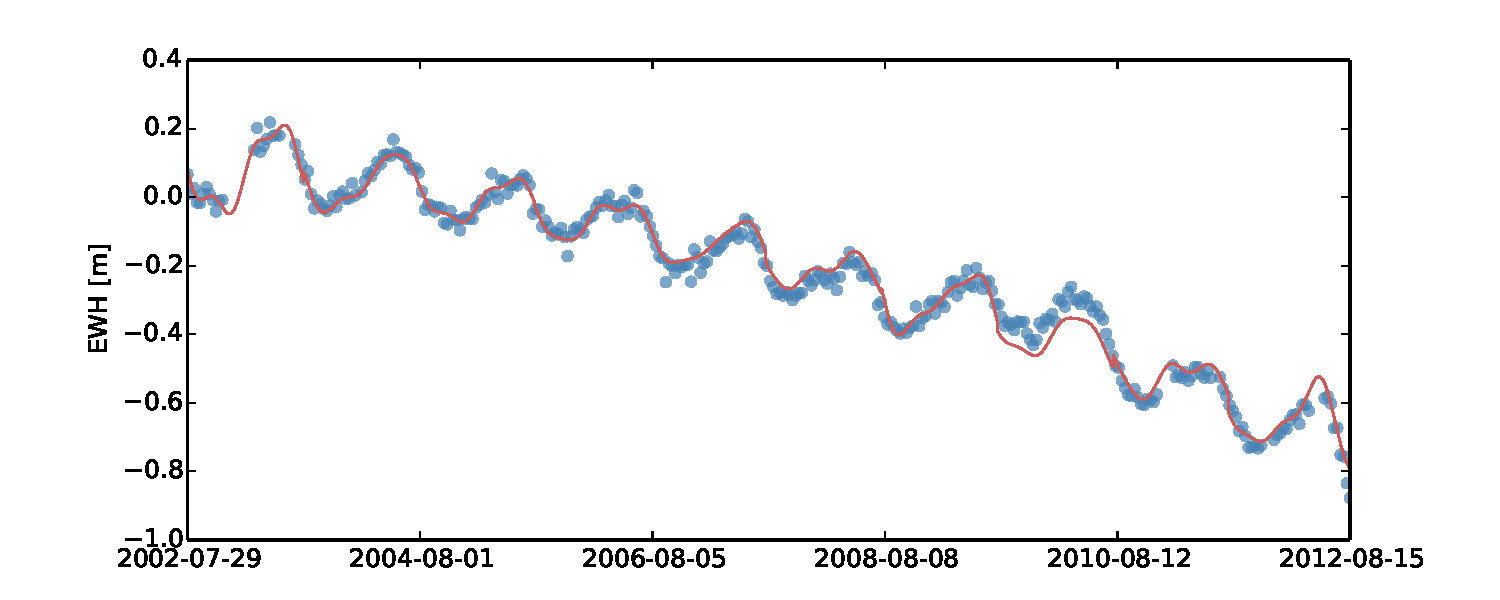
\includegraphics[width=\textwidth]{figures/splines-selected-0-fit}
	\caption{Measurements are blue, the OLS fit is red.}
	\label{fig:splines-selected-0-fit}
\end{figure}

\begin{figure}[H]
	\centering
	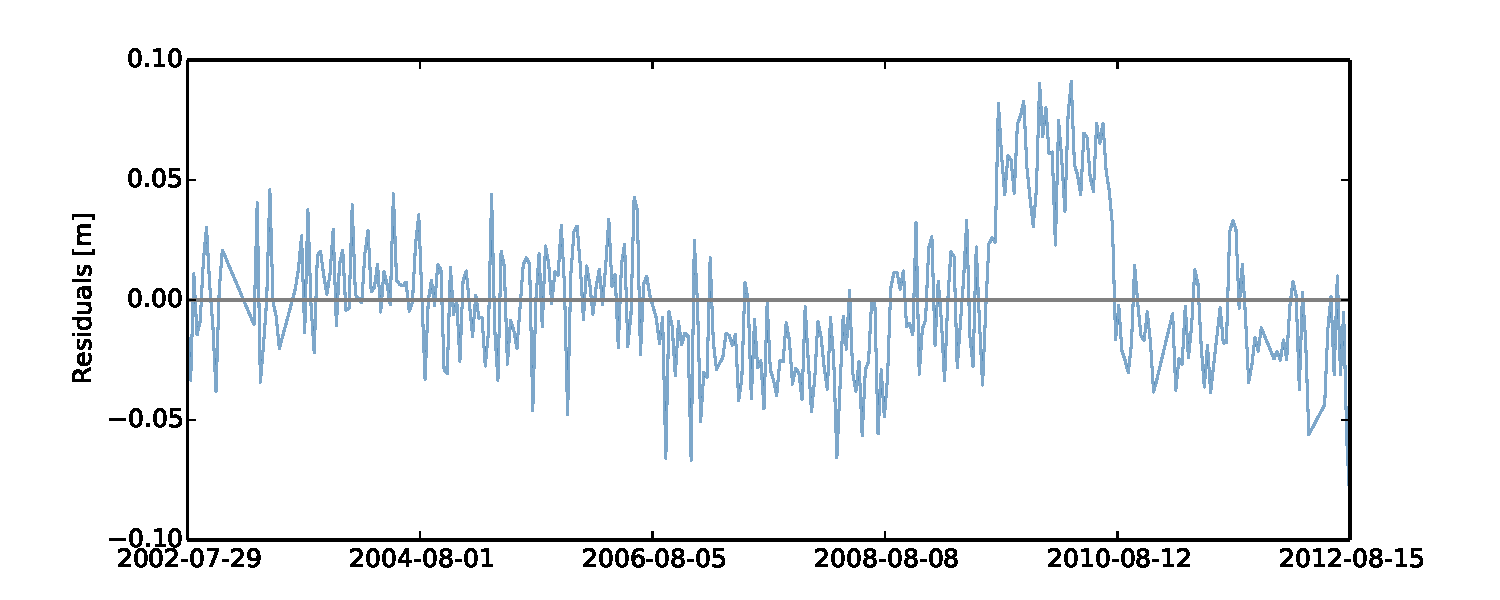
\includegraphics[width=\textwidth]{figures/splines-selected-0-residual}
	\caption{The OLS residuals are blue.}
	\label{fig:splines-selected-0-residual}
\end{figure}

Unfortunately for the south pole, the resulting fits do display some cusps and overfitting behavior. This is particularly seen at 2006 and 2008. Here the residuals haven't improved much, however interestingly enough there now appear to be a two year seasonal trend, between 2003 and 2007. 

\begin{figure}[H]
	\centering
	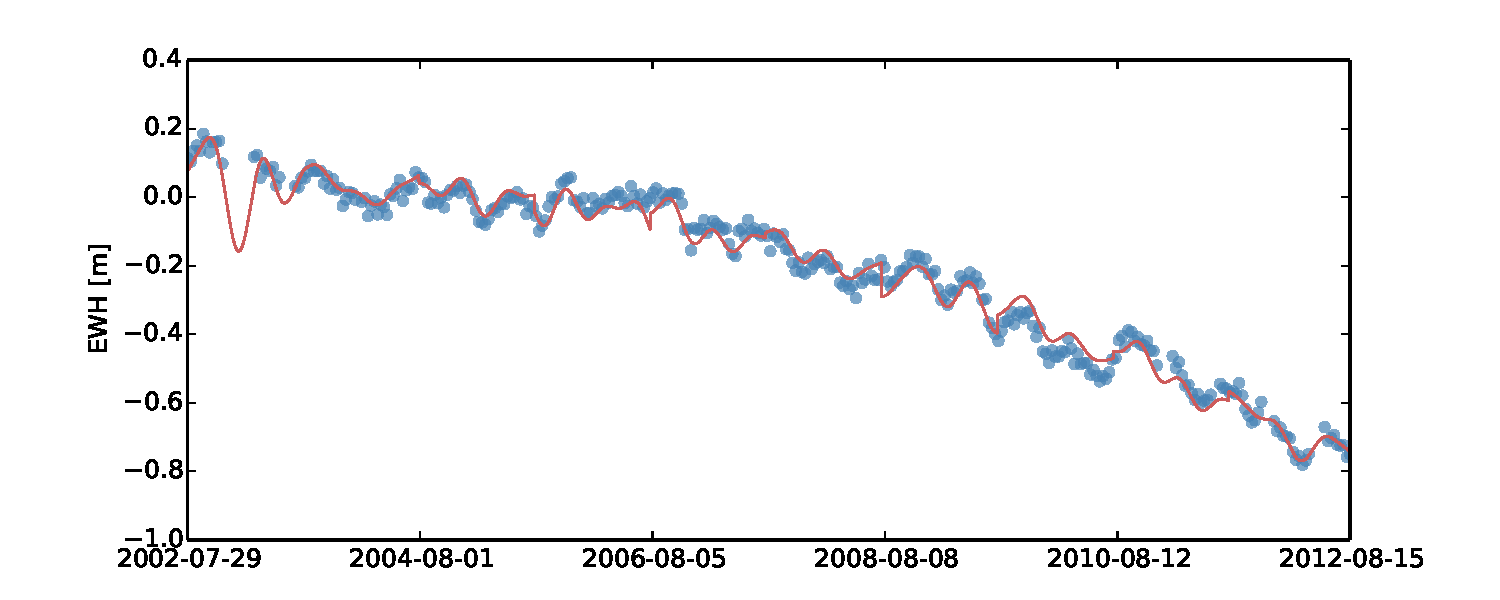
\includegraphics[width=\textwidth]{figures/splines-selected-1-fit}
	\caption{Measurements are blue, the OLS fit is red.}
	\label{fig:splines-selected-1-fit}
\end{figure}

\begin{figure}[H]
	\centering
	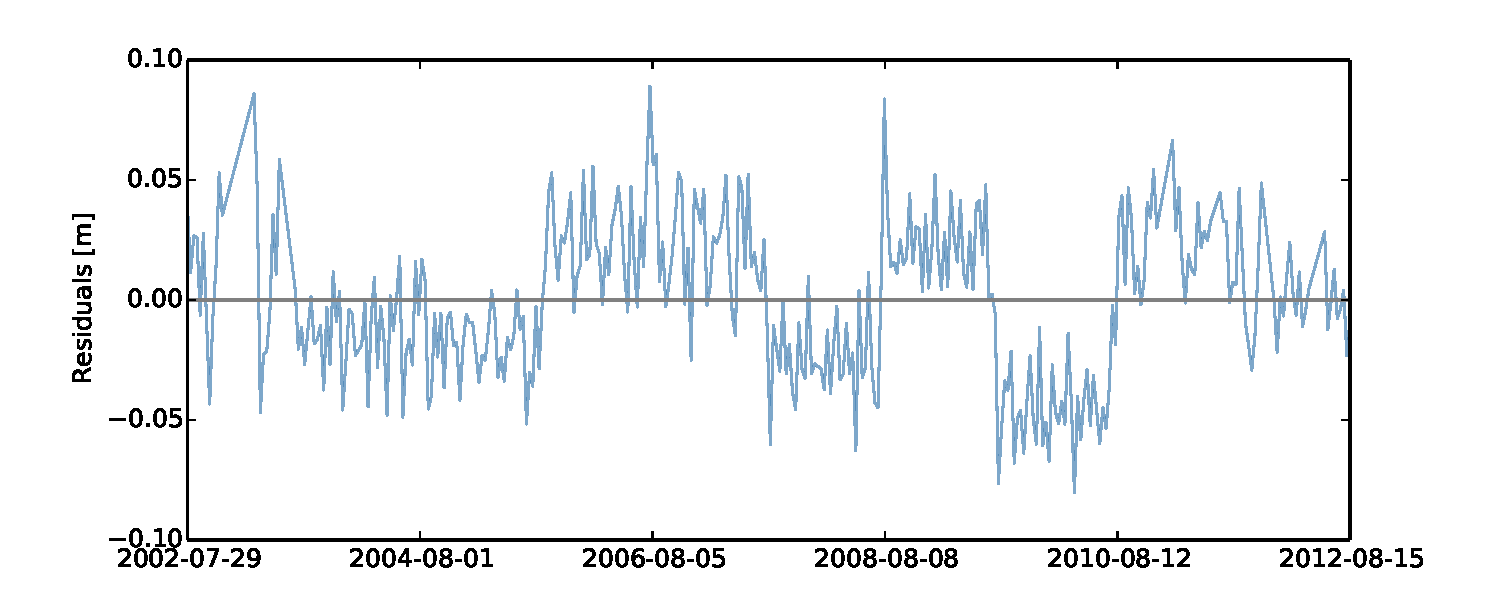
\includegraphics[width=\textwidth]{figures/splines-selected-1-residual}
	\caption{The OLS residuals are blue.}
	\label{fig:splines-selected-1-residual}
\end{figure}

\subsubsection{Ideas}
If one wanted to delve deeper into the possibilities of basis expansions and hinge function the most important thing would be to analyse where to place the knots. Even though it was here chosen to place the knots at predetermined points in time and have the knots be equal for all locations, several libraries have been developed which optimizes knot location as well polynomial degrees etc.
 A famous algorithm MARS\textregistered (multivariate adaptive regression splines) developed by Jerome Friedman, can achieve this using a 2-phase pass technique \cite{wiki-MARS} (forward, backward) but implementing the algorithm seemed out of scope for this report.
\todo[inline]{Andreas er uenlig. Den slags er brugtbart når man forventer pludselige hendelser, men ikke ved hvornår. Som fx US Air Trafic. I vores tilfælde giver det perfekt mening at modeller en svingning til et år. At introducere en ny svinging (et år) før den forige er gennemføret, gør modellen urealistisk. Istedet bør man fokusere på de curps der er nu, da det er det umidbare problem. Dette løser MARS heller ikke.}
